
As explained in Section~\ref{sec:introduction}, the term \enquote{trending} denotes the alignment of a detected true development with the development indicated by another measurement, a nowcast, or a forecast.
In this section, we want to specify trending and define different methods of measuring and visualizing trending.
In general, trending can be assessed for different lags $l$ separately, and the relevance of the considered lags has to be determined based on the question at hand.
Throughout the section, we call a measurement, nowcast, or forecast a \textit{prediction} or \textit{signal} whenever the application area is insignificant.
Before introducing measures to evaluate trending, we make remarks on calculating the predicted change and notation in Section~\ref{subsec:notation}.
Section~\ref{subsec:trending-basics} introduces trending basics and visualizes trending in a synthetic example.
In Section~\ref{subsec:trending-measures}, various methods from other disciplines and tasks are applied and examined.
The approaches are extended to account for noise and non-systematic effects in Section~\ref{subsec:trending-noise}.
Section~\ref{subsec:trending-cond-prob} introduces a new graphical method for local trending assessment and briefly introduces bootstrap methods for computing confidence intervals for the measures in the previous sections.
Trending assessment for probabilistic nowcasts and forecasts is treated in Section~\ref{subsec:probabilistic}.

\subsection{Computing the predicted change and notation}\label{subsec:notation}

As noted above, trending refers to observed and predicted changes for a time lag $l$.
The \textit{observed} change is straightforward to compute for all types of signals.
Let $\mathbf{y} = (y_t)_{t=0}^T$ denote the true values for nowcasting or forecasting, or gold standard measurements up to time $T$.
The sequence of observed change is then given by the differences of values in $\mathbf{y}$ with lag $l$, that is
\begin{equation}\label{eq:diffy}
    \diffylt = (y_{t+l} - y_t) \quad \text{for}\ t = 1, \dots, T - l.
\end{equation}


As noted in the introduction, the definition of the predicted change depends on the context.
Applying the computation for $y$ directly, the signal's predicted change would be the difference between the signal at time $t + l$ and the true value at $t$.
This approach lags in three practical aspects.
For nowcasting and forecasting, the true value at time $t$ might not be known with a considerable time delay.
In the nowcasting application of Section~\ref{sec:application-covid}, for example, the time delay is more than 80 days.
Until the true values are publicly available, the change cannot be computed, and no actions can be taken based on it.
Thus, using updated signal values for time $t$ as the reference value in this setting is more practically relevant.

Second, in the context of nowcasting or forecasting, several signals for the same time $t + l$ are often available at different generation times.
Thus, the generation time and forecast time have to be included in the notation of nowcasts and forecasts.
We use the term \textit{issue time} for the generation time of a signal and \textit{target time} to denote the time the forecast applies to.

Third, for measurement, a test method is usually evaluated against a gold standard to test whether the test method could replace the gold standard.
Thus, the gold standard measurements are not available if the quality of the test method is sufficient. \improvement{irgendwie für mich nicht klar formuliert: man unteruscht ja bei meausurement nur ob die gemessenen Änderungen von den zwei Methoden konsistent sind oder?}
Thus, the predicted change is computed based on the values of the test method at time $t$ and $t + l$.

Taking the three points together, the signal's predicted change is based on the type of signal.
To account for several signals for a target time $t$ at different issue times $\tau$, we denote them by $x_{t | \tau}$.
For nowcasting, target times $t$ are usually not considerably later than issue times $\tau$, while $t$ is usually at least $\tau$ in forecasting. For measurements, this distinction is not necessary.
Table~\ref{tab:notation} summarizes the notation for the different signal types and the computation of the predicted change.

\begin{table}
    \centering
    \begin{tabularx}{0.75\textwidth}{l X}
        \toprule
        Application & Predicted change computation \\
        \midrule
        Measurement & $(x_{t + l} - x_t)_{t=1}^T \label{eq:diffxl_measure} $\\
        Nowcasting & $
\diffxl =
\begin{cases}
(x_{t+l|t+l} -x_{t|t+l})^T_{t=1} & \text{if } y_{t} \text{ is not known at time } t, \\
(x_{t+l|t+l} -y_{t})^T_{t=1} & \text{else}.
\end{cases} \label{eq:diffxl_nowcasting}
$ \\
        Forecasting & $
\diffxl =
\begin{cases}
(x_{t+l|t} - x_{t|t})^T_{t=1} & \text{if } y_{t} \text{ is not known at time } t, \\
(x_{t+l|t} - y_{t})^T_{t=1}  & \text{else}.
\end{cases} \label{eq:diffxl_forecasting}
$\\
        \bottomrule
    \end{tabularx}
    \caption{Computation of the predicted change in the different applications. Signals $x_{t | \tau}$ refer to values issued at $\tau$ with a target time $t$. Note the different relations between the issue and target time for nowcasts and forecasts. }
    \label{tab:notation}
\end{table}


\subsection{Basics of trending and four-quadrant plots}\label{subsec:trending-basics}

Although the calculation of $\diffxl$ differs in different contexts, the trending assessment is similar.
In the following, we omit the difference lag $l$ for ease of notation; $\diffx$ and $\diffy$ refer to $\diffxl$ and $\diffyl$ for a common lag $l$ as defined in Table~\ref{tab:notation}.
As noted above, a signal's trending is perfect if all the change directions are predicted correctly; that is, the sign of all elements of $\diffx$ and $\diffy$ coincide.
Perfect trending is hardly the case in practice, but a weaker requirement is needed.
Consequently, when evaluating the trending, we examine the statistical consistency of $\sign(\diffx)$ and $\sign(\diffy)$.
A simple yet insightful method is the four-quadrant plot.
For example, it is known in cardiac output measurement analysis~\parencite{Saugel2015,perrino1998intraoperative}. 
Thus, the occured changes are plotted with the predicted changes, that is, $(\diffy_t, \diffx_t)$ for $t = 1, \dots, T$.
Thus, the x-axis of a four-quadrant plot shows the true value differences, whereas the y-axis displays the prediction data differences.
Points in the green upper right and lower left quadrants reflect a correct trending for the respective time step, whereas points in the remaining red quadrants show incorrect predicted changes.

Figure~\ref{fig:trending_basic_4q} displays a basic four-quadrant plot.
Points 2, 3, 5, and 6 show trending, whereas points 1, 4, and 7 count for anti-trending behavior.
Figure~\ref{fig:trending_basic_4q_sample} shows a four-quadrant graph for a more extensive simulated data set with $T=1461$, for example, four years of daily data.
Data generation is described in Appendix~\ref{subsec:app-trending-data-generation} and will continue into this section.
The four-quadrant plot resembles a butterfly-like shape, with more data in the upper right and lower left quadrants than in the remaining quadrants.

The four-quadrant plot is intuitive to interpret, and the magnitude and direction of change are shown simultaneously.
It can be extended by including information on the date in the point color.
In Figure~\ref{fig:trending_basic_4q_sample_color}, the point colors turn from blue to green for higher time indices $t$.
The lag is always one time step.
However, four-quadrant plots become crowded for larger datasets, and sequential information on the differences is complex to assess thoroughly.
There are other visualization techniques, such as polar plots or the Bland-Altmann analysis.
However, they lack the four-quadrant plot's clarity and intuition without adding more information on trending~\parencite{Saugel2015}.

\begin{figure}
\centering
\begin{subfigure}[t]{.24\textwidth}
\includegraphics{plots/illustrative_examples/4Q_without_excl}
\caption{Basic four-quadrant plot.} \label{fig:trending_basic_4q}
\end{subfigure}\hspace{0.01\textwidth}%
\begin{subfigure}[t]{.24\textwidth}
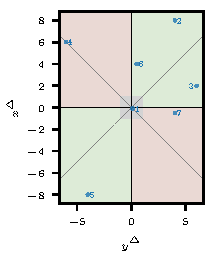
\includegraphics{plots/illustrative_examples/4q_excl_box}
\caption{Four-quadrant plot with rectangular exclusion area.}\label{fig:trending_basic_4q_excl_box}
\end{subfigure}\hspace{0.01\textwidth}%
\begin{subfigure}[t]{.24\textwidth}
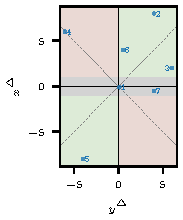
\includegraphics{plots/illustrative_examples/4q_excl_axis}
\caption{Four-quadrant plot with horizontal exclusion area.} \label{fig:trending_basic_4q_excl_axis}
\end{subfigure}\hspace{0.01\textwidth}%
\begin{subfigure}[t]{.24\textwidth}
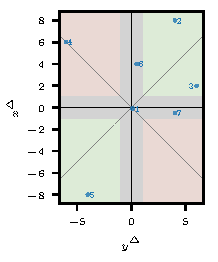
\includegraphics{plots/illustrative_examples/4q_excl_cross}
\caption{Four-quadrant plot with cross-shaped exclusion area.}\label{fig:trending_basic_4q_excl_cross}
\end{subfigure}%
\caption{Illustrations of the four-quadrant plot with sample points and with and without exclusion areas. }
\label{fig:trending_4q}
\end{figure}

\subsection{Trending ratio and other measures}\label{subsec:trending-measures}

Analyzing the number of points in the green versus red quadrants is a standard approach in the trending assessment of measurement data \parencite{Critchley2010,Saugel2015}. 
It boils down to assessing the probability of trending $P(\diffxrv \diffyrv > 0)$, where $\diffyrv$ and $\diffxrv$ denote random variables for future incremental changes.
Note that $z_1 z_2 > 0$ if and only if $\sign(z_1) = \sign(z_2)$ ($z_1, z_2 \in \R \setminus \{ 0 \}$).
The standard estimator for $P(\diffxrv \diffyrv > 0)$ is
\begin{equation}
    \acc (\diffx, \diffy) \coloneqq \frac{\sum_{t \in \mathcal{T}} \ind{\diffxt \diffyt > 0}}{\card{T}}.\label{eq:acc}
\end{equation}
We refer to this estimator as the trending ratio of the prediction and set $\mathcal{T} = \{1, \dots, T-l\}$.
Visually, the measure computes the fraction of points in the upper right or lower left quadrant.
Such a $2 \times 2$ table of counts is called a contingency table.
It is often used in other scientific areas for evaluation, for example, in dichotomous forecasting or as a confusion matrix in classification analysis~\parencites(see, e.g., the introductions in)()[Ch. 4]{James2021}[Ch. 3]{Jolliffe2012}.
There, a wide range of other methods are usually used to analyze further characteristics of contingency tables.
Two simple measures that focus on specific areas of interest are the positive and negative trending ratios $\accp$ and $\accm$, respectively.
They are defined as
\begin{align}
    \accp (\diffx, \diffy) &\coloneqq \frac{\sum_{t \in \mathcal{T}} \ind{\diffxt \diffyt > 0} \ind{\diffxt > 0}}{\sum_{t \in \mathcal{T}} \ind{\diffxt > 0}} \label{eq:accp}\\
    \accm (\diffx, \diffy) &\coloneqq \frac{\sum_{t \in \mathcal{T}} \ind{\diffxt \diffyt > 0} \ind{\diffxt < 0}}{\sum_{t \in \mathcal{T}} \ind{\diffxt < 0}}\label{eq:accm}
\end{align}
In the classification context, these measures are known as positive or negative predictive value and hit rate or detection failure ratio in forecasting.
They give the probability of a correct prediction of the direction of change, given that the signal direction is positive or negative, respectively.
Therefore, they measure the trending ability of the prediction for positive and negative changes separately by cutting the considered data.
In terms of probability, the two measures give estimates of $P(\diffxrv \diffyrv > 0 | \diffxrv > 0)$ and $P(\diffxrv \diffyrv > 0 | \diffxrv < 0)$, respectively.

Using these estimators could encourage predictors to exploit imbalances in the number of positive and negative changes. 
A large difference in $\sum_{t \in \mathcal{T}} \ind{\diffyt > 0}$ and $\sum_{t \in \mathcal{T}} \ind{\diffyt < 0}$ is unlikely in the trending setting, as $\diffy$ is obtained from differencing time series data. 
However, if the number of positive and negative $\diffy$ differs widely, the use of unbalanced-data-aware measures should be considered.
There are various adapted measures for unbalanced outcomes, for example, Cohen's $\kappa$ \parencite{Cohen1960} or those listed in \textcite[Table 3.3]{Jolliffe2012}.
Cohen's $\kappa$ is usually used to measure inter-rater agreement and considers the ratio of occurred agreement and the probability of agreement by chance.
Cohen's $\kappa$ reduces to rescaling the trending ratio for a $2\times2$-table and balanced outcomes.

All measures can also be evaluated as a rolling estimate to detect changes in performance over time.
A rolling estimate is a sequence of estimates, each computed on a length-$w$-window of the data.
For the trending ratio, a rolling estimate with a backward-looking window is given by
\begin{equation*}
    \acc_t (\diffx, \diffy) \coloneqq \frac{\sum_{t^\star = t-w + 1}^{t} \ind{\diffxt[t^\star] \diffyt[t^\star] > 0}}{w}, \quad t = w-1, \dots, T.\label{eq:acc_rolling}
\end{equation*}
Figure~\ref{fig:trending_ratio_time_series} depicts a rolling window estimate of the trending ratio for the simulated data of Figures~\ref{fig:trending_basic_4q_sample} and~\ref{fig:trending_basic_4q_sample_color}.
Thus, the yearly course of the prediction trending ratio can be detected.
The trending ability of the signal has a strong sinus-shaped seasonality with a trending ability peak after a quarter of a year and a low point after three quarters.
This seasonal behavior cannot be distinguished in the two four-quadrant plots or the trending ratio.


\begin{figure}
    \centering
    \begin{subfigure}[t]{.24\textwidth}
\includegraphics{plots/illustrative_examples/4Q_sample_without_time}
\caption{Four-quadrant plot with simulated data.}\label{fig:trending_basic_4q_sample}
\end{subfigure}\hspace{0.01\textwidth}
\begin{subfigure}[t]{.24\textwidth}
\includegraphics{plots/illustrative_examples/4Q_sample_with_time}
\caption{The same data is colored according to the time index $t$, the greener, the later.}\label{fig:trending_basic_4q_sample_color}
\end{subfigure}\hspace{0.01\textwidth}
\begin{subfigure}[t]{.48\textwidth}
    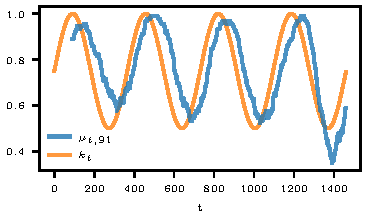
\includegraphics{plots/illustrative_examples/trending_ratio_time_series.pdf}
    \caption{Rolling estimate of the trending ratio over time with window length 91. }\label{fig:trending_ratio_time_series}
    \end{subfigure}%
    \caption{Visualizations for data with a time-varying trending ratio. We defer information on the data generation process in \ref{fig:trending_basic_4q_sample} and \ref{fig:trending_basic_4q_sample_color} to the appendix (see \ref{subsec:app-trending-data-generation}). The trending ratio for the entire data set is $\mu = 0.7577$. The strong seasonality of the trending ratio becomes visible in Figure~\ref{fig:trending_ratio_time_series}. The green curve $k_t$ shows the probability that $\diffxt$ has the same sign as $\diffyt$ for each time step. The rolling estimates are delayed as the windows look backward.}
\end{figure} 

In applications, signal data are often not available for all time steps, for example, due to technical problems or delays in data transfer (see the examples in Sections~\ref{sec:application-covid} and~\ref{sec:application-eda}).
We refer to time steps for which either signal or true values or both are unavailable as missing values.
Data pairs with missing values can be excluded from the set $\mathcal{T}$ to calculate the measures. 
However, systematical missing values could lead to a biased estimate of the trending ratio, for example, if signal data is omitted in times of high change and thus uncertainty.
In this case, measures should be interpreted cautiously, and
inspection of missing data should accompany applications with missing data, for example, through a visual assessment.
In the applications in Sections~\ref{sec:application-covid} and~\ref{sec:application-eda}, only a few missing values occur, and we provide information on the missing data by inspecting the missing data as lists.

\subsection{Accounting for noise and non-informative small changes}\label{subsec:trending-noise}

The above measures use only information on a point's quadrant and neglect further details on its location within the quadrant.
However, points close to the zero point have intuitively less explanatory power or are less reliable.
Suppose noise or non-systematic effects are present in the true values or predictions. In that case, a point's assignment to a quadrant can be driven by noise instead of a systematic trending ability of the signal.
This happens more frequently for points with at least one small coordinate.

Using an exclusion area around the zero point is a straightforward and highly interpretable extension of the measures of Section~\ref{subsec:trending-measures}.
Points within that area are neither plotted in the four-quadrant plot nor included in the calculation of the measures.
The shape of the exclusion area can be chosen according to the noise characteristics of the predictions and the true values.
In general, it is likely that the prediction models have a noise component and should thus be part of the exclusion area.
We denote the measures of Equations~\eqref{eq:acc},~\eqref{eq:accp} and~\eqref{eq:accm} accounting for an exclusion area $E$ by
\begin{align}
    \acceps (\diffx, \diffy, E) &\coloneqq \frac{\sum_{t \in \mathcal{T}} \ind{\diffx \diffy > 0} \ind{(\diffyt, \diffxt) \notin E}}{\sum_{t \in \mathcal{T}} \ind{(\diffyt, \diffxt) \notin E}}\label{eq:acceps}\\
    \accpeps (\diffx, \diffy, E) &\coloneqq \frac{\sum_{t \in \mathcal{T}} \ind{\diffxt \diffyt > 0} \ind{\diffxt > 0, , (\diffyt, \diffxt) \notin E}}{\sum_{t \in \mathcal{T}} \ind{\diffxt > 0, (\diffyt, \diffxt) \notin E}} \label{eq:accpeps}\\
    \accmeps (\diffx, \diffy, E) &\coloneqq \frac{\sum_{t \in \mathcal{T}} \ind{\diffxt \diffyt > 0} \ind{\diffxt < 0, (\diffyt, \diffxt) \notin E}}{\sum_{t \in \mathcal{T}} \ind{\diffxt < 0, (\diffyt, \diffxt) \notin E}}\label{eq:accmeps}
\end{align}
The measures are then estimators for the probability of trending, given that the change is not in the exclusion area $E$, that is, for $\acceps$, $P(\diffxrv \diffyrv > 0 | \diffxrv \diffyrv \notin E)$.
The estimators accept various shapes of the exclusion area.
Figure~\ref{fig:trending_4q} visualizes different shapes of the exclusion area.
A rectangular exclusion area, $E = \{(x, y) \in \R^2: (-\varepsilon_x \leq x \leq \varepsilon_x) \land (-\varepsilon_y \leq y \leq \varepsilon_y) \}$ 
 ($\varepsilon_x, \varepsilon_y > 0$), leaves out points that are small in both components and, therefore, likely to be driven by noise.
Points where at least the true value or signal is unlikely to be zero are not excluded.
In the example graph in Figure~\ref{fig:trending_basic_4q_excl_box}, only point 1 is excluded.
An exclusion area along one axis, for example, $E = \{(x, y) \in \R^2: (-\varepsilon_x \leq 0 \leq \varepsilon_x)\}$ for $\varepsilon_x > 0$, removes points in which one of the components could change sign by a small amount of noise.
This particularly suits signals where small amounts of noise are inevitable.
A cross-shaped exclusion area, $E = \{(x, y) \in \R^2: (-\varepsilon_x \leq x \leq \varepsilon_x) \lor (-\varepsilon_y \leq y \leq \varepsilon_y) \}$ for $\varepsilon_x, \varepsilon_y > 0$, along both axes accounts for the sign reversal in both components.
For these two methods, points 1 and 7 in Figure~\ref{fig:trending_basic_4q_excl_axis} or 1, 6, and 7 are excluded in Figure~\ref{fig:trending_basic_4q_excl_cross}, respectively.

In addition to these straight shapes, exclusion areas could have more complex shapes, such as ellipses.
Such a shape could, for example, be obtained by using a multivariate normal error model around the zero point and excluding points that exceed a certain likelihood of being produced by chance from the zero point.
These shapes are theoretically appealing, but interpreting the resulting estimators becomes complex.
Thus, we suggest using the above simple exclusion areas.

In most applications, the shape and size of the exclusion area can be chosen based on domain knowledge or expert opinions.
The size estimation can also be based on a proportion of the total variance or the total range of the data.
A third approach is to visualize the trending ratio for different sizes of $E$ and thus inspect the effects of the exclusion area size on the estimates.


\subsection{Bootstrap confidence intervals and the conditional trending plot}\label{subsec:trending-cond-prob}
\unsure{Vielleicht doch zwei subsections?}
Confidence intervals can account for the estimation uncertainty of the measures above.
Bootstrap confidence intervals are a nonparametric technique based on resampling~\parencite[for introductions see][]{Hesterberg2011,Bittmann2021}.
New samples are drawn with replacement from the dataset and are not based on parametric assumptions as classical confidence intervals are.
The confidence interval is then computed based on the bootstrap samples.
We examine three methods for bootstrapping: the intuitive percentile and the more sophisticated basic and \ac{bca} method.
In the \textit{percentile} approach, the confidence interval for the level $\alpha$ is built directly from the empirical distribution of the bootstrap estimators.
The \textit{basic} approach computes the confidence interval based on the non-bootstrap estimate using the bootstrapped quantile deviations~\parencite{Davison1997}.
The \ac{bca} method modifies the quantiles of the empirical bootstrap distribution by a bias and an acceleration parameter~\parencite{Efron1987}.
Typically, the percentile approach needs larger datasets and provides an easy and fast estimate, while the \ac{bca} is computationally expensive but requires smaller datasets for reasonable confidence intervals.
The basic approach balances these two objectives.
We compare the approaches in a small synthetic data study on their small-dataset behavior and computation time in Appendix~\ref{sec:appendix-trending}.
\Ac{bca} is the only method that maintains the confidence level also for small datasets while increasing the computation time only moderately for larger datasets.
Therefore, we use the \ac{bca} method for confidence intervals in the applications in Section~\ref{sec:application}.

The sample is assumed to be independent and identically distributed in standard bootstrapping.
Thus, before applying bootstrapping methods, the strength of sequential dependence should be inspected, for example, by analyzing the autocorrelation and partial autocorrelation.
The simple bootstrapping methods above do not account for serial dependence. 
Bootstrapping focusing on time series data is covered in~\textcite{Hardle2003,Kreiss2012}, for example.

The estimators described above give information on the probabilities $P(\diffxrv \diffyrv > 0 | \diffxrv \diffyrv \notin e)$, $P(\diffxrv \diffyrv > 0 | \diffxrv > 0, \diffxrv \diffyrv \notin e)$ and $P(\diffxrv \diffyrv > 0 | \diffxrv < 0, \diffxrv \diffyrv \notin e)$.
These probabilities draw a general picture but might still be too coarse for local effects.
More insights might be gained by considering the conditional distribution to assess the local trending ability of a prediction.
While it would be possible to build analog measures for other intervals, assessing $P(\diffxrv \diffyrv > 0 | \diffx = x)$ graphically eases the simultaneous evaluation of various intervals.
Furthermore, the graph facilitates the comparison of various methods in a single graph and asymmetries of $P(\diffxrv \diffyrv > 0 | \diffx = x)$ with respect to $x$ in the trending ability can be detected.
We refer to the plot as a conditional trending plot.

A multivariate \acf{kde} facilitates a continuous estimation of $P(\diffxrv \diffyrv > 0 | \diffxrv = x)$ by estimating the components $f_{\diffxrv, \diffyrv}$ and $f_{\diffxrv}$ of
\begin{align*}
P(\diffxrv \diffyrv > 0 | \diffxrv = x) = \begin{cases}
                                              \int_{-\infty}^0 \frac{f_{\diffxrv, \diffyrv}(x, y)}{f_{\diffxrv}(x)} \ \textrm{d} \: y & \text{if } x < 0, \\
                                              \int_{0}^{\infty} \frac{f_{\diffxrv, \diffyrv}(x, y)}{f_{\diffxrv}(x)} \ \textrm{d} \: y & \text{if } x > 0, \\
\end{cases}
\end{align*}
for $x \neq 0$ through a \ac{kde}.

A comprehensive introduction to multivariate \ac{kde} can be found in \textcite{Gramacki2018}, and implementations are available in many programming languages~\parencite[e.g., for  Python in][]{Seabold2010}.
The \ac{kde} yields estimates for $P(\diffxrv \diffyrv > 0 | \diffxrv = x)$ for all values of $x \in \R$.
Multivariate \ac{kde} takes a kernel and bandwidth selector as modeling parameters. 
The kernel is usually Gaussian, and there are multiple methods for selecting the bandwidth, each with its advantages and disadvantages.
Note that for kernels with infinite support, for example, the Gaussian kernel, the plot should be limited to the core values of $\diffx$ without outliers to avoid estimates based on small subsets of the data.

Figure~\ref{fig:trending-cond-prob-bw} shows the resulting conditional trending plots for the three well-known selectors, rule-of-thumb, cross-validation maximum likelihood, and cross-validation least squares using the \verb|statsmodels| Python package~\parencite{Seabold2010}.
While the rule-of-thumb is based only on the covariance matrix, the other two numerically optimize the bandwidth with a hold-one-out least squares or likelihood objective function.
The dashed line shows the theoretical $P(\diffyrv \diffxrv > 0 | \diffxrv = x)$.
The second method, cross-validation least squares, requires long computation times while yielding small or no bandwidth results, even for two relatively small datasets.
The rule-of-thumb and cross-validation maximum likelihood methods yield reasonable results at moderate computation times. 
Further examples, including comparisons between methods regarding their trending ability, are available in Section~\ref{sec:application}.

\begin{figure}
    \centering
    \begin{subfigure}{.48\textwidth}
        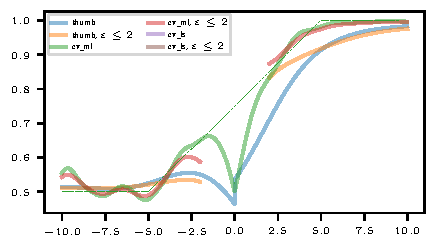
\includegraphics{plots/illustrative_examples/cond_prob_plot_bw_asym_butterfly}
        \caption{First dataset with asymmetric dependence.}
    \end{subfigure}
    \begin{subfigure}{.48\textwidth}
        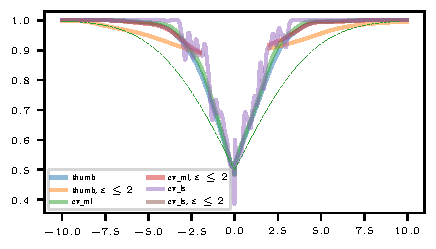
\includegraphics{plots/illustrative_examples/cond_prob_plot_bw_normal}
        \caption{Second dataset. }
    \end{subfigure}
    \caption{Resulting conditional trending plot for different bandwidth selection processes. Cross-validation least squares takes a considerably larger computation time. It does not converge for the first data set and yields a bandwidth too small for the second data set. The rule of thumb is the fastest method but tends to oversmooth. The cross-validation maximum likelihood method yields a more reasonable bandwidth with moderate computation time. }\label{fig:trending-cond-prob-bw}
\end{figure}

\newpage
\subsection{Probabilistic Evaluation}\label{subsec:probabilistic}

In nowcasting and forecasting, there is a shift from point predictions to probabilistic predictions (see, for example, Sections~\ref{sec:application-covid} and~\ref{sec:application-eda} or the review in~\cite{Gneiting2014}).
Probabilistic predictions include a point estimate and information on the forecast uncertainty and quantiles simultaneously.
In this section, we extend the trending assessment to probabilistic predictions.

Probabilistic predictions can take the form of a \ac{cdf}, \ac{pdf}, or quantiles.
The \ac{cdf} is the most general and can be used to derive the others, given they exist.
Let us first assume that the prediction is a \ac{cdf} and the lag is large enough to know the true value when issuing the forecast or nowcast.
See the end of the section for predictions given as quantiles or for unknown true values.

Let $F_{t | \tau} (x)$ denote the predicted \ac{cdf} of forecast time $t$ and issue time $\tau$, where the index is analogous to the point prediction notation of Section~\ref{subsec:notation}.
For trending assessment, we compare the probability of positive change with the occurrence of positive changes. 
The probability $p_t$ of a positive change is given by one minus the \ac{cdf} of the prediction at the true value at the issue time. 
As for the differences in Section~\ref{subsec:notation}, the computation differs slightly for nowcasts and forecasts.
For nowcasts, the probability is calculated by
\begin{equation*}
    p_t = 1 - F_{t+l | t+l} (y_{t})\quad t = 1, \dots, T-l;
\end{equation*}
while for forecasts, it is given by
\begin{equation*}
    p_t = 1 - F_{t+l | t} (y_{t})\quad t = 1, \dots, T-l.
\end{equation*}
Let $z_t$ denote the indicator that the observed change at time $t$ is positive, that is,
\begin{equation*}
    z_t = \ind{\diffyt > 0} \quad t = 1, \dots, T-l.
\end{equation*}
The probabilistic trending evaluation is then based on the probabilities $\mathbf{p} = (p_t)_{t=1}^{T-l}$ and the observed changes $\mathbf{z} = (z_t)_{t=1}^{T-l}$.
The predictive power of $\mathbf{p}$ for $\mathbf{z}$ can be assessed using probabilistic dichotomous forecast evaluation methods.
Dichotomous forecasts predict a binary outcome, for example, a positive or negative change.
Numerical measures for forecast quality are scoring rules.
The \ac{bs} is a widely used scoring rule for dichotomous probabilistic forecasts~\parencite{Brier1950}.
It is defined as
\begin{equation*}
    BS (\mathbf{p}, \mathbf{z}) = \frac{1}{T-l} \sum_{t=1}^{T-l} (p_t - z_t)^2.
\end{equation*}
The \ac{bs} assesses the calibration and sharpness of the forecast and the observation simultaneously~\parencite{Ranjan2010,Mitchell2011}.
Calibration refers to the statistical consistency of forecasts and observations, while sharpness measures the spread of the forecast distribution.
A smaller spread, and thus, higher sharpness, is preferable, as it indicates greater confidence in the prediction.
The basic paradigm of probabilistic forecasting is to maximize sharpness, subject to calibration~\parencite{Gneiting2014}.
These two conflicting aspects cannot be distinguished in the scoring rule.

Graphical models are a standard tool for evaluating solely the calibration of probabilistic forecasts.
In dichotomous forecasting, the reliability diagram is frequently used~\parencite{Ranjan2010}.
The reliability diagram plots the observed frequency of the positive outcome against the predicted probability.
Ideally, the predicted probability equals the observed frequency, and the reliability diagram is a 45-degree line.
Local deviations from the 45-degree line indicate a miscalibration of the forecast for specific probabilities.
Thus, the reliability visualizes the local and overall calibration simultaneously.
For an example of a reliability diagram, see Section~\ref{sec:application-eda}.

If forecasts or nowcasts are given as quantiles, $p_t$ can be determined by interpolations among the quantiles.
Let $q_p$ denote the quantiles for forecast time $t+l$ for even-spaced probabilities $p \in \{1/\pmax, \dots, (p-1) / \pmax\}$ ($\pmax \in \N \setminus \{1, 2\}$) and $y_t$ the true value at time $t$. \unsure{ist das richtig?}
The quantiles $q_p$ generally differ for each time step, but we omit an index here for ease of notation.
The probability $\pc_t$ of a \textit{negative} change is between $p^{\star}$ and $p^{\star} + 1/\pmax$ for
\begin{equation*}
    p^{\star} = \max \{p \in \{1/\pmax, \dots, (\pmax-1) / \pmax\}: q_p \leq y_t\} , \quad \text{if}\ q_{1/\pmax} \leq y_t \leq q_{1 - 1/\pmax}.
\end{equation*}
Quantiles do not determine the location within the interval $[p^{\star}, p^{\star} + 1/\pmax]$.
Under the assumption of a uniform distribution within the quantile interval, the probability of a negative change is
\begin{equation*}
    \bar{p}_t = \frac{y_t - q_{p^\star}}{\pmax (q_{p^{\star} + 1} - q_{p^{\star}})} + p^{\star}.
\end{equation*}
The approach does not assign probabilities for $y_t$ smaller than the smallest quantile $q_{1/p}$ or larger than the largest quantile.
As a simple extension, we assume that the probability mass is uniformly distributed on an interval of the same length as the nearest interval specified by the quantiles.
This yields
\begin{equation*}
\bar{p}_t = \begin{cases}
    \max \{\frac{1}{\pmax} - \frac{q_{p^\star} - y_t}{\pmax (q_{p2/\pmax} - q_{1/\pmax})}, 0\} &, \text{if } y_t < q_{1/p}, \\
    \min \{\frac{1}{\pmax} - \frac{y_t - q_{(\pmax-1)/\pmax}}{\pmax (q_{(\pmax-1)/\pmax} - q_{(\pmax-2)/\pmax})}, 1\} &, \text{if } y_t > q_{1 - 1/p}, \\
    \frac{y_t - q_{p^\star}}{\pmax (q_{p^{\star} + 1} - q_{p^{\star}})} + p^{\star} &, \text{otherwise.}
\end{cases}
\end{equation*}
The probability of positive change is $p_t = 1 - \bar{p}_t$.

If the true value is given as a distribution because it is still unknown, the probabilities $p_t$ can be computed by integration.
Let for two nowcasts the distributions be given by \acp{pdf} $f_{t+l|t+l}$ and $f_{t|t+l}$ with \acp{cdf}  $F_{t+l|t+l}$ and $F_{t|t+l}$.
Then, the probability of a negative change can be computed by
\begin{align}
    \bar{p}_t
        &= \int_{\begin{subarray}{l}x_1, x_2 \in \R: \\ x_2 < x_1\end{subarray}} f_{t|t+l} (x_1) f_{t+l|t+l} (x_2)  \ \textrm{d} \: (x_1, x_2) \nonumber\\
        &= \int_{x_1 \in \R} \int_{-\infty}^{x_1} f_{t|t+l} (x_1) f_{t+l|t+l} (x_2)  \ \textrm{d} \: x_2 \ \textrm{d} \: x_1 \nonumber\\
        &= \int_{x_1 \in \R} f_{t|t+l} (x_1) F_{t+l|t+l} (x_1)  \ \textrm{d} \: x_2 \ \textrm{d} \: x_1 \label{eq:trending-probabilistic-pdf}.
\end{align}
\unsure{Die Unabhängigkeitsannahme ist nicht zu streng? weil es ist ja eigentlich die Aufgabe von einenm guten Nowcaster diese Abhängigkeit zu modellieren oder?}
Thereby, the distributions are assumed to be independent.
If the nowcasts have the form of a multivariate distribution, including the dependence of the two \acp{pdf}, $f_{t+l|t+l} (x_2)$ has to be replaced by the \ac{pdf} conditional on $x_1$.
As a Monte Carlo approximation of Equation~\eqref{eq:trending-probabilistic-pdf}, the probability can also be calculated by sampling from $f_{t+l|t+l}$ and $f_{t|t+l}$ and calculating the fraction of negative changes.
For forecasts, the indexes have to be shifted.
If no \acp{pdf} are available, they can be estimated from the \ac{cdf} or quantiles, or the \ac{cdf} or quantiles can be used to generate samples for the Monte Carlo approximation.
